\ylDisplay{Liikumine} % Ülesande nimi
{Autor} % Autor
{lõppvoor} % Voor
{2011} % Aasta
{P 2} % Ülesande nr.
{1} % Raskustase
{
% Teema: Mehaanika

\ifStatement
Graafikul on kujutatud liikuva keha kiiruse sõltuvust ajast. Kui suur oli vaadeldava aja jooksul keha suurim kaugus algasendist? Kui kaugel oli keha algasendist vaadeldava ajavahemiku lõpus?
\begin{center}
	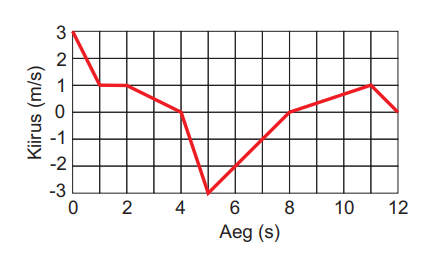
\includegraphics[width=0.5\linewidth]{2011-v3p-02-yl.PNG}
\end{center}
\fi

\ifHint
Ülevalpool ajatelge olev graafiku joon kirjeldab liikumist positiivses suunas, allpool ajatelge olev joon negatiivses suunas. Kuna liikumise iseloom igal etapil on erinev, tuleb arvutada iga etapi jooksul läbitud teepikkus arvestades ka liikumise suunda. Teepikkust võib arvutada graafiku joone ja ajatelje vahelise pindala kaudu.
\fi

\ifSolution
Ülevalpool ajatelge olev graafiku joon kirjeldab liikumist positiivses suunas, allpool ajatelge olev joon negatiivses suunas. Kuna liikumise iseloom igal etapil on erinev, tuleb arvutada iga etapi jooksul läbitud teepikkus arvestades ka liikumise suunda. Teepikkust võib arvutada graafiku joone ja ajatelje vahelise pindala kaudu. Kuna enamjaolt on tegemist ühtlaselt muutuva liikumisega, võib teepikkuse leida ka seose
\begin{center}
$s = \frac{v+v_0}{2} t$ abil. 
\end{center}
Keha on algpunktist kõige kaugemal neljanda sekundi lõpus, s.o. $4$ $m$ kaugusel. Keha lõpetab liikumise samas punktis, kus alustas.
\fi
}

